%===================================================================================
% Chapter: Propuesta para la Extracción de Entidades
%===================================================================================
\chapter{Propuesta para la Extracción de Entidades}\label{chapter:entities}
\addcontentsline{toc}{chapter}{Extracción de Entidades}
%===================================================================================

%===================================================================================

En este capítulo se hace una descripción de las técnicas empleadas para la resolución de la tarea de Extracción de Entidades, donde se describe como funciona el modelo de aprendizaje profundo propuesto, la construcci\'on de su entrada a partir de una oraci\'on, entre ellas la obtenci\'on de los \emph{Embeddings Contextuales} de las palabras de una oraci\'on hacienqdo uso de \textbf{BERT}. Finalmente se describe cada una de las componentes del modelo de aprendizaje profundo y su funcionamiento.


\section{Modelo de Aprendizaje Profundo}

El modelo propuesto es un \emph{BiLSTM-CRF} apilado que tiene como entrada \emph{Embeddings Contextuales} pre-entrenados con \textbf{BERT}, \emph{Postag Embeddings} que son entrenados junto al modelo y \emph{Char Embeddings} que se entrenan junto al modelo a partir de una \textbf{CNN}. El modelo tiene como decodificador para la predicci\'on de las etiquetas correspondientes a cada token un \textbf{CRF}. El modelo pretende determinar cu\'ales son las entidades dentro de la oraci\'on y de esas entidades cu\'al es su clasificaci\'on como \emph{Concepto}, \emph{Acci\'on}, \emph{Predicado} y \emph{Referencia}.

\subsection{Entrada del Modelo}\label{sec:entrance}
Se recibe como entrada una oraci\'on en texto plano, la cual necesita preprocesamiento para construir la entrada apropiada del modelo. El primer paso es tokenizar las oraciones dado que todas las entradas del modelo esperan una secuencia de tokens. Para esto se utiliza la tokenizaci\'on por espacios y basada en reglas.

Por cada token en el cual una oraci\'on fue dividida, la entrada respectiva a ese token consiste de una lista de tres vectores de rasgos.

\begin{description}
	\item[Vector de PoS-tag:] Es un vector \emph{one-hot} de codificaci\'on de la informaci\'on de \emph{Part of Speech} (\textbf{PoS}).
	\item[Codificaci\'on de los caracteres:] Es la concatenaci\'on de los vectores \emph{one-hot} de codificaci\'on de cada uno de los caracteres contenidos en la palabra. 
	\item[Embedding Contextual:] Es un vector de \emph{embedding} de la palabra conformado por la concatenaci\'on de los vectores que representan a dicha palabra en cada una de las capas de \textbf{BERT}.
	 
\end{description} 

Para obtener la \emph{Codificaci\'on de los caracteres} se utiliz\'o el alfabeto (VER COMO DESCRIBIMOS EL ALFABETO). Para extraer la informaci\'on de \textbf{PoS-tag} se utiliza la librer\'ia de python \textbf{spacy}~\footnote{spacy.io}. 

Para la construcci\'on de los \emph{Emmbeddings Contextuales} correspondientes a cada token se utiliza \textbf{BERT}, siguiendo el siguiente procedimiento. Se toma la oraci\'on y se le agregan al inicio y al final las cadenas de texto \emph{"[CLS]"} y \emph{"[SEP]"} respectivamente. Luego esta nueva oraci\'on es tokenizada utilizando un algoritmo de tokenizaci\'on de subpalabras conocido como \emph{Word Piece}~\cite{schuster2012japanese}. El vocabulario de \emph{Word Piece} de \textbf{BERT} se computa aplicando el algoritmo de \emph{Word Piece tokenization} en cada secuencia de caracteres del corpus en el que se entren\'o \textbf{BERT}: \emph{Wikipedia and the Book Corpus}, lo cual resulta en 30 mil tokens de vocabulario. Como es l\'ogico, debido al tipo de tokenizaci\'on \emph{Word Piece}, se quisiera distinguir dentro del vocabulario a las palabras \emph{venoso} como una sola palabra y el sufijo \emph{venoso}, por lo que el sufijo se representa de la forma \emph{\#\#venoso} en el vocabulario.

%por el \emph{BertTokenizer} de la biblitoeca \textbf{pytorch-pretrained-bert}~\footnote{https://pypi.org/project/pytorch-pretrained-bert/} utilizando un algoritmo de tokenizaci\'on de subpalabras conocido como \emph{Word Piece}~\cite{schuster2012japanese}. 

%La tokenizaci\'on de \emph{Word Piece} es en esencia la idea de un algoritmo de compresi\'on, en este caso de representar palabras frecuentes con menos s\'imbolos y palabras menos frecuentes con m\'as s\'imbolos lo cual es de hecho la idea que hay detr\'as de varios esquemas de codificaci\'on como la codificaci\'on de \emph{Huffman}. \emph{Word Piece aplica el mismo principio} y t\'ecnicas a la tokenizaci\'on. \emph{Word Piece} es un algoritmo \emph{bottom- up} para la tokenizaci\'on de subpalabras que aprende un vocabulario de subpalabras de cierto tama\~no. La idea b\'asica es la siguiente:
%
%\begin{enumerate}
%	\item Comienza separando todas las palabras en caracteres unicode. Cada caracter unicode corresponde a un s\'imbolo en el vocabulario final. Se comienza con este vocabulario minimalista y luego se expande.
%	\item Mientras a\'un haya espacio en el vocabulario se hace lo siguiente:
%	\begin{enumerate}
%		\item Encontrar la pareja (\emph{bigram}) de s\'imbolos tal que al mezclarla incrementa the likelihood de un modelo de lenguaje unigram entrenado en los datos de entrenamiento. Este tipo de mezcla adem\'as de la frecuencia de la pareja de s\'imbolos, tiene en cuenta la frecuencia de los s\'imbolos del vocabulario inicial que los conforman. La log likelihood de una oraci\'on en una modelo de lenguaj unigram (asumiendo independencia entre las palabras) es la suma de las frecuencias de los s\'imbolos que los componen. Esto significa que mezclar dos s\'imbolos incrementa el total de la log likelihood por el log likelihood de los dos s\'imbolos mezclados y disminuir por los log likelihod de los dos s\'imbolos originales. Asumiendo que se mezclan \emph{x} y \emph{y}, el incremento en el log likelihood total ser\'ia de:
%		
%		\begin{equation}
%			\log p(x,y) - \log p(x) - \log p(y) = \log \frac{\log(p(x))}{\log(p(x))\log(p(y))}
%		\end{equation}
%		
%		\item Mezclar esos dos s\'imbolos para crear un nuevo s\'imbolo y a\~nadirlo al vocabulario. Esto incrementa el tama~no del vocabulario en 1.
%	\end{enumerate}
%	
%\end{enumerate} 

Posteriormente los tokens obtenidos tras tokenizar la oraci\'on utilizando el \emph{Word Piece tokenizer} son llevados a \'indices con respecto al vocabulario de \textbf{BERT}. Adem\'as se contruye la m\'ascara de atenci\'on poniendo a todos los tokens el valor de \textbf{1}, dado que no es necesario para nuestros objetivos hacer \emph{padding} de las oraciones. Luego la secuencia de \'indices de los tokens en el vocabulario de \textbf{BERT} y la m\'ascara de atenci\'on son pasadas como entrada del modelo pre-entrenado de \textbf{BERT}, obteniendo as\'i como salida la codificaci\'on de cada una de las capas de \textbf{BERT}.

Luego el \emph{Embedding Contextual} de cada token se construye a partir de la concatenaci\'on de la codificaci\'on de dicho token en las \textbf{n} capas de \textbf{BERT}, o sea, si el token \textbf{t}, tiene codificaciones $l_1, l_2, ..., l_n$ en cada una de las capas de \textbf{BERT} respectivamente, entonces el \emph{Embedding Contextual} del token \textbf{t} ser\'ia la concatenaci\'on de cada una de las codificaciones anteriores, resultando en el vector: $l_1l_2....l_n$.

Sin embargo, debido a la tokenizaci\'on del tipo \emph{Word Piece} realizada, hay palabras que quedan separadas en varios tokens, como por ejemplo \emph{[c\'an], [\#\#cer]}, donde la palabra \emph{c\'ancer} es una entidad y se clasificar\'ia como \emph{Concepto}, pero para que la arquitectura del modelo de aprendizaje profundo para resolver \textbf{NER} pueda etiquetar correctamente a la palabra c\'ancer tendr\'ia que etiquetar dos tokens en vez de uno, por eso para la entrada del modelo de aprendizaje profundo para resolver la \emph{Subtarea A} se utiliza el tokenizer por espacios y basado en reglas no el \emph{Word Piece Tokenizer}. Por lo que queda el problema de que al obtener, del modelo pre-entrenado de \textbf{BERT}, los \emph{Embeddings Contextuales} de cada uno de los tokens obtenidos de la \emph{Word Piece tokenization} es necesario computar cu\'al ser\'ia el \emph{Embedding Contextual} de los tokens obtenidos por la tokenizaci\'on por espacios basada en reglas. Luego para obtener un vector de \emph{Embedding Contextual} para los tokens obtenidos por la tokenizaci\'on por espacios basada en reglas se hace un algoritmo de \textbf{mapping}. 

Para las palabras que son un solo token en el tokenizer por espacios y basado en reglas, pero en el \emph{Word Piece Tokenizer} son m\'as de uno como por ejemplo \emph{c\'ancer} y \emph{[c\'an], [\#\#cer]} respectivamente, se hace una mezcla de los \emph{Embeddings Contextuales}. Por ejemplo si el token \emph{[c\'an]} tiene \emph{Embedding Contextual x} y el token \emph{[\#\#cer]} tiene \emph{Embedding Contextual y}, entonces el \emph{Embedding Contextual} del token \emph{c\'ancer} ser\'ia la mezcla de \emph{x} y \emph{y}. De forma general sea $T_b$ un tokenizer por espacios y basado en reglas y sea $T_{wp}$ un \emph{Word Piece tokenizer} y sea $w$ una palabra en una oraci\'on tal que $T_b$ tiene a $w$ como un token por si sola, mientras que para $T_{wp}$ existe un \textbf{k} tal que $w$ se descompone en \textbf{k}- tokens, luego de la palabra $w$ se obtienen en $T_{wp}$ los tokens $t_1, t_2, ..., t_k$, donde para cada uno de los tokens $t_1, t_2, ..., t_k$ se obtiene un \emph{Embedding Contextual} $e_1, e_2, ..., e_k$ a partir de la concatenaci\'on de la codificaci\'on de cada uno de los tokens en todas las capas de \textbf{BERT}. Luego sea $v$ un vector de \emph{embeddings} de dimensi\'on \textbf{k} y sea $f(v)$ una funci\'on de mezcla que recibe un vector de dimensi\'on \textbf{k} y retorna un \'unico \emph{embedding}, entonces el \emph{Embedding Contextual} del token $w$ del tokenizer $T_b$ es el resultado de aplicar $f$ al vector conformado por los \emph{Embeddings Contextuales} $e_1, e_2, ..., e_k$. Si denotamos $E(t)$ como una funci\'on que recibe un token y devuelve su \emph{Embedding contextual}, y $V = <e_1, e_2, ..., e_k>$ como el vector de dimensi\'on \textbf{k} que contiene los \emph{Embeddings Contextuales} de los tokens $t_1, t_2, ..., t_k$, entonces:

\begin{equation}
	E(w) = f(V)
\end{equation}

Particularmente se utiliz\'o como funci\'on de mezcla $f$ el promedio de los vectores de \emph{Embedding Contextual}.

\subsection{Arquitectura del Modelo}

El modelo recibe una secuencia de tokens como entrada como fue descrito en~\ref{sec:entrance}. La arquitectura se divide en tres niveles: (1) representaci\'on de los \emph{tokens}, (2) respresentaci\'on de la secuencia, y (3) predicci\'on de las etiquetas \emph{BMEWO-V} y la clasificaci\'on seg\'un las etiquetas \emph{Concept}, \emph{Action}, \emph{Reference}, \emph{Predicate} y \emph{None}, esta \'ultima en caso de no pertenecer a ninguna de las anteriores. La figura~\ref{fig:ArcMod} y sdfsdf resumen la arquitectura del modelo.


\begin{figure}[h!]
	\centering
	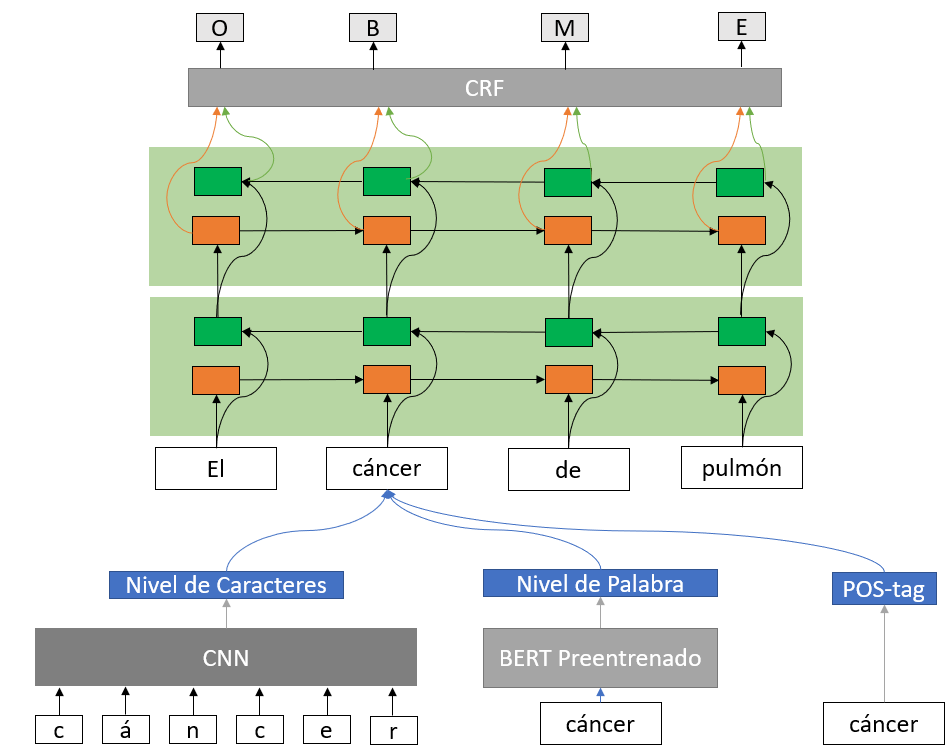
\includegraphics[width = 10cm]{Imagenes/EntitiesModelRec.png}
	\caption{Arquitectura del modelo de aprendizaje profundo para la extraccio\'on y clasificaci\'on de entidades con el CRF para la decodificaci\'on de las etiquetas \emph{BMEWO-V}.}\label{fig:ArcMod}
\end{figure}

\begin{figure}[h!]
	\centering
	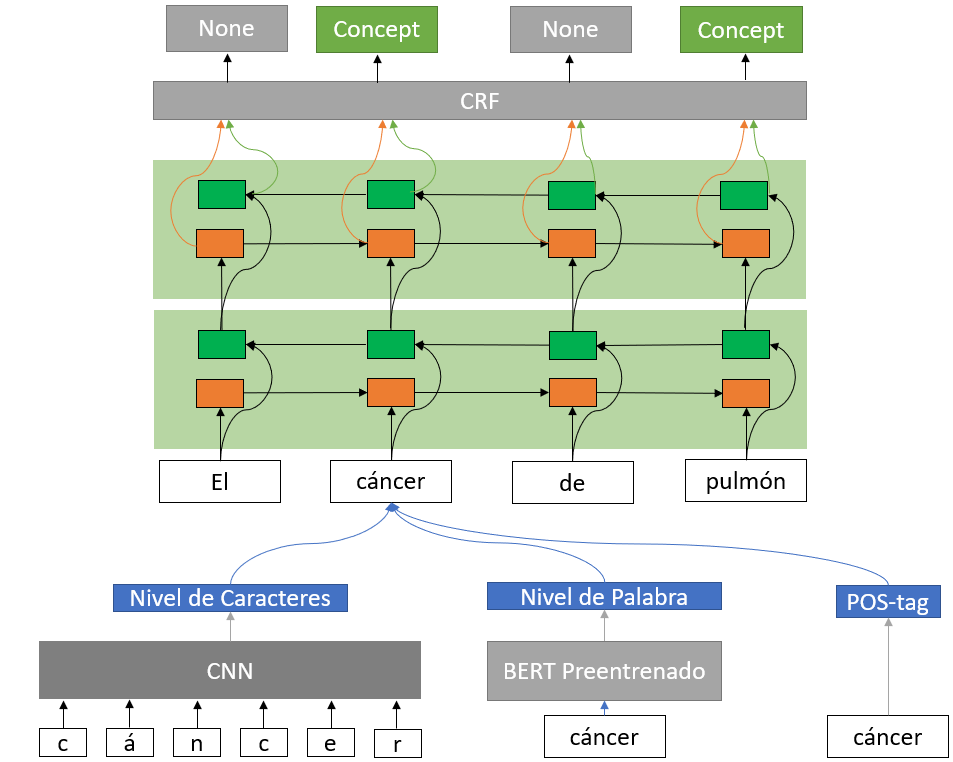
\includegraphics[width = 10cm]{Imagenes/EntitiesModelClas.png}
	\caption{Arquitectura del modelo de aprendizaje profundo para la extraccio\'on y clasificaci\'on de entidades con el CRF para la decodificaci\'on de las etiquetas de clasificaci\'on \emph{Concept}, \emph{Action}, \emph{Reference}, \emph{Predicate} y \emph{None},}\label{fig:ArcMod}
\end{figure}

En un primer nivel, el modelo se encarga de obtener la representaci\'on de cada token en la secuencia de entrada, para ello existe una capa intermedia que trabaja en funci\'on de transformar la caracter\'istica \emph{Char Indexes} en vectores, que junto al de \emph{PosTag} y el \emph{Embedding Contextual} forman la representaci\'on final del token. Una capa \textbf{CNN} convierte los \emph{Char Indexes} en un vector de \emph{embedding} que atrapa el significado sem\'antico del token a nivel de caracteres. Esto se incluye para que el modelo se auxilie de caracter\'isticas morfol\'ogicas de la palabra (como prefijos y sufijos) en caso de que el token no forme parte del vocabulario del \textbf{BERT} pre-entrenado. El vector obtenido a partir de la \textbf{CNN} concatenado con el vector de \emph{Embedding Contextual} y el de \emph{PosTag} forman la representaci\'on del token.

En un segundo nivel, el modelo procesa la secuencia de tokens para obtener representaciones a nivel de oraci\'on. Una capa \emph{Bi-LSTM} recorre la secuencia de tokens en ambos sentidos para construir dos secuencias de vectores. Los vectores en posiciones complementarias de las dos secuencias son concatenados, obteni\'endose as\'i nuevamente una secuencia que asocia un vector dependiente del contexto, que captura informaci\'on de la oraci\'on completa, a cada token de la oraci\'on. Esta secuencia busca atrapar las dependencias semánticas entre los tokens de la oración.
Luego una segunda \emph{Bi-LSTM} apilada, que se utiliza tradicionalmente para a\~nadir m\'as poder representacional, recorre la secuencia devuelta por la primera \emph{Bi-LSTM} en ambos sentidos, para tambi\'en construir dos secuencias de vectores que son concatenadas, produciendo as\'i otra nueva secuencia que asocia un vector a cada token de la oraci\'on capturando informaci\'on m\'as compleja que la obtenida por la primera capa \emph{Bi-LSTM}.

En el \'ultimo nivel, existen dos capas \emph{CRF} para la decodificaci\'on de etiquetas. La primera capa \emph{CRF} utiliza la representaci\'on obtenida del nivel anterior para predecir la secuencia de etiquetas \emph{BMEWO-V}. Mientras la segunda capa \emph{CRF} utiliza la representaci\'on obtenida del nivel anterior para predecir para cada token de la secuencia su clasificaci\'on como \emph{Concept}, \emph{Action}, \emph{Reference}, \emph{Predicate} y\emph{None} en caso que no sea ninguna de las anteriores.

\subsection{Postprocesamiento}
(PONER EL POSTPROCESAMIENTO RALIZADO A LA SALIDA DEL MODELO)
La capa de CRF produce una clasificaci\'on acorde al sistema \emph{BMEWO-V} de etiquetado. Dicho sistema clasifica cada \emph{token} en \emph{B} para inicio de palabra clave, \emph{M} para continuaci\'on de palabra clave, \emph{E} para fin de palabra clave, \emph{W} para las palabras clave formadas por un solo \emph{token} y \emph{O} para los \emph{token} que no representan nada. Adem\'as, contempla la posibilidad de solapamiento entre palabras clave mediante la etiqueta \emph{V}. 
\newline
\newline
Este sistema es adaptado al escenario del \emph{IberLEF 2019}, donde se clasifican las palabras clave en \emph{Concepto}, \emph{Acci\'on}, \emph{Referencia} o \emph{Predicado}. Para ello, cada etiqueta \emph{B}, \emph{M}, \emph{E}, \emph{W} se sufija con \emph{Concepto}, \emph{Acci\'on}, \emph{Referencia} o \emph{Predicado} de acuerdo al tipo de palabra clave (la etiqueta \emph{V} puede o no tenerlo). La salida del modelo es una secuencia de estas etiquetas sufijadas. 
\newline
\newline
Para convertir la secuencia de etiquetas sufijadas que se obtiene de la oraci\'on dada, se realiza un procedimiento iterativo por la misma. Dicho procedimiento asume que el nivel de solapamiento entre palabras clave es menor o igual que dos. Esta suposici\'on, dada por las limitaciones del sistema \emph{BMEWO-V}, es lo que provoca mayor error de recobrado en este procedimiento. Dado esto, se mantienen durante la iteraci\'on los \emph{spans} de texto de las dos palabras clave que en potencia se est\'an construyendo. Estos dos objetos son actualizados en cada iteraci\'on de acuerdo a la etiqueta actual y la anterior. La etiqueta \emph{B} indica el inicio de una palabra clave, la \emph{M} la extensi\'on de la palabra clave que ya existe y la \emph{E} su finalizaci\'on. La etiqueta \emph{V} introduce un solapamiento, luego esta es la etiqueta que puede provocar que en alg\'un momento existan dos palabras clave en construcci\'on. La etiqueta \emph{W} causa que se reporte autom\'aticamente la existencia de una palabra clave en el \emph{span} de texto asociado a la misma. Luego de identificada una palabra clave, para clasificarla se utiliza un sitema de votaci\'on. Cada etiqueta que haya formado parte de una palabra clave que se report\'o como tal, "vot\'o" para decidir si era \emph{Concepto}, \emph{Acci\'on}, \emph{Referencia} o \emph{Predicado}, en correspodencia con su sufijo asociado. Cuando se reporta la palabra clave se clasifica de acuerdo a la mayor cantidad de votos que haya obtenido. Si est\'a equilibrada la votaci\'on se asume \emph{Concepto}.



















